\begin{name}
	{\tenchude}
	{ĐỀ TT CHUYÊN QUANG TRUNG - BÌNH PHƯỚC}
	{LỚP TOÁN THẦY PHÁT}
	{Chi sa aspettare, ottiene ciò che vuole}
\end{name}
\caulc
\Opensolutionfile{ans}[ans/ans\currfilebase]
%Câu 1
\begin{ex}%[2D1N1-2]%[Dự án đề KTTT Môn Toán KSCL NH25-26 - Dot 6 - Trần Tiến Đức]%[ChuyenQuangTrung-BinhPhuoc]%[GVPB Nguyễn Sĩ Đạt]	
	Biết hàm số $y=\dfrac{x+a}{x-1}$ (a là số thực cho trước, $a\ne-1$) có đồ thị như trong hình vẽ sau:
	\begin{center}
		\begin{tikzpicture}[scale=0.8, font=\footnotesize, line join=round, line cap=round, >=stealth]
			\draw[->] (-3,0)--(4,0) node [below]{$x$};
			\draw[->] (0,-3)--(0,4) node [left]{$y$};
			\node at (0,0) [below left]{$O$};
			
			\draw[dashed] (-3,1)--(4,1);
			\draw[dashed] (1,-3)--(1,4);
			
			\begin{scope}
				\clip (-3,-3) rectangle (4,4);
				\draw[samples=150,smooth,variable=\x, domain=-3:0.85] plot (\x,{(\x-2)/(\x-1)});
				\draw[samples=150,smooth,variable=\x, domain=1.15:4] plot (\x,{(\x-2)/(\x-1)});
			\end{scope}
			
		\end{tikzpicture}
	\end{center}
	Mệnh đề nào dưới đây đúng?
	\choice
	{$y'<0 , \forall x\in\mathbb{R}$}
	{$y'<0 , \forall x\ne 1$}
	{\True $y'>0 , \forall x\ne 1$}
	{$y'>0 , \forall x\in\mathbb{R}$}
	\loigiai{
		Dựa vào đồ thị hàm số ta thấy hàm số đồng biến trên các khoảng $(-\infty;1)$ và $(1;+\infty)$.\\
		Do đó hàm số đã cho có $y'>0 , \forall x\ne1$.
	}
\end{ex}

%Câu 2
\begin{ex}%[2D1N1-2]%[Dự án đề KTTT Môn Toán KSCL NH25-26 - Dot 6 - Trần Tiến Đức]%[ChuyenQuangTrung-BinhPhuoc]%[GVPB Nguyễn Sĩ Đạt]	
	Cho hàm số $y=f(x)$ xác định trên $\mathbb{R} \backslash \{-1\}$, có bảng xét dấu của đạo hàm như hình vẽ. Hàm số đã cho nghịch biến trên khoảng nào dưới đây?
	\begin{center}
		
\begin{tikzpicture}
			\tkzTabInit[nocadre=false,lgt=1.2,espcl=2.5,deltacl=0.6]
			{$x$/0.6, $f'(x)$/0.8}
			{$-\infty$, $-1$, $1$, $+\infty$}
			\tkzTabLine{ , -, d, -, 0, +, }
		\end{tikzpicture}
	\end{center}
	\choice
	{$(1;+\infty)$}
	{$(-\infty;1)$}
	{$(-1;+\infty)$}
	{\True $(-\infty;-1)$}
	\loigiai{
		Dựa vào bảng biến thiên của hàm số $y=f(x)$ ta thấy hàm số nghịch biến trên khoảng $(-\infty;-1)$.
	}
\end{ex}

%Câu 3
\begin{ex}%[2D1N4-1]%[Dự án đề KTTT Môn Toán KSCL NH25-26 - Dot 6 - Trần Tiến Đức]%[ChuyenQuangTrung-BinhPhuoc]%[GVPB Nguyễn Sĩ Đạt]	
	Cho hàm số $y=f(x)$ có bảng biến thiên như sau:
	\begin{center}
		
\begin{tikzpicture}
			\tkzTabInit[nocadre=false,lgt=1.2,espcl=2.5,deltacl=0.6]
			{$x$/0.6, $f'(x)$/0.6, $f(x)$/2}
			{$-\infty$, $0$, $1$, $+\infty$}
			\tkzTabLine{ , +, 0, -, d, +, }
			\tkzTabVar{-/ $0$, +/ $2$, -D-/ $-\infty$ / $3$, +/ $5$}
		\end{tikzpicture}
	\end{center}
	Tổng số tiệm cận ngang và tiệm cận đứng của đồ thị hàm số đã cho là
	\choice
	{$4$}
	{$2$}
	{\True $3$}
	{$1$}
	\loigiai{
		Dựa vào bảng biến thiên của hàm số $y=f(x)$ ta thấy
		$\lim\limits_{x\rightarrow-\infty}f(x)=0$; $\lim\limits_{x\rightarrow+\infty}f(x)=5$.\\
		Suy ra đồ thị hàm số có hai tiệm cận ngang là $y=0$; $y=5$.\\
		Lại có $\lim\limits_{x\rightarrow1^{-}}f(x)=-\infty$ nên đồ thị hàm số có tiệm cận đứng $x=1$.\\
		Vậy đồ thị hàm số đã cho có tổng cộng $3$ tiệm cận.
	}
\end{ex}

%Câu 4
\begin{ex}%[2D4N3-1]%[Dự án đề KTTT Môn Toán KSCL NH25-26 - Dot 6 - Trần Tiến Đức]%[ChuyenQuangTrung-BinhPhuoc]%[GVPB Nguyễn Sĩ Đạt]	
	Cho đồ thị hàm số $y=f(x)$ như hình vẽ. Gọi $S$ là diện tích của hình phẳng giới hạn bởi đồ thị $y=f(x)$ và trục $Ox$ . Tìm khẳng định sai.
	\begin{center}
		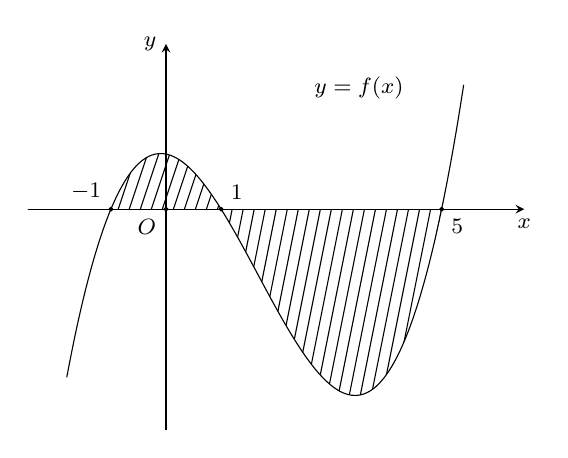
\begin{tikzpicture}[scale=0.7, font=\footnotesize, line join=round, line cap=round, >=stealth]
			\begin{scope}
				\clip (-1,0) -- plot[domain=-1:1, samples=100] (\x, {0.2*(\x+1)*(\x-1)*(\x-5)}) -- (1,0) -- cycle;
				\foreach \i in {-2,-1.8,...,2} \draw (\i,-1) -- (\i+1,2);
			\end{scope}
			\begin{scope}
				\clip (1,0) -- plot[domain=1:5, samples=100] (\x, {0.2*(\x+1)*(\x-1)*(\x-5)}) -- (5,0) -- cycle;
				\foreach \i in {0,0.2,...,6} \draw (\i,-4) -- (\i+1,1);
			\end{scope}
			
			\draw[->] (-2.5,0)--(6.5,0) node [below]{$x$};
			\draw[->] (0,-4)--(0,3) node [left]{$y$};
			\node at (0,0) [below left]{$O$};
			\draw[fill=black] (0,0) circle(1pt);
			
			\draw[samples=100, smooth, variable=\x, domain=-1.8:5.4] 
			plot (\x, {0.2*(\x+1)*(\x-1)*(\x-5)});
			\node at (-1,0) [above left]{$-1$};
			\node at (1,0) [above right]{$1$};
			\node at (5,0) [below right]{$5$};
			\draw[fill=black] (-1,0) circle(1pt);
			\draw[fill=black] (1,0) circle(1pt);
			\draw[fill=black] (5,0) circle(1pt);
			\node at (3.5,2.2) {$y=f(x)$};
			
		\end{tikzpicture}
	\end{center}
	\choice
	{\True $S=\displaystyle\int\limits_{-1}^{1}f(x)\,\mathrm{\,d}x+\displaystyle\int\limits_{1}^{3}f(x)\,\mathrm{\,d}x$}
	{$S=\left|\displaystyle\int\limits_{-1}^{1}f'(x)\,\mathrm{\,d}x \right|+\left|\displaystyle\int\limits_{1}^{5}f'(x)\,\mathrm{\,d}x \right|$}
	{$S=\displaystyle\int\limits_{-1}^{1}f(x)\,\mathrm{\,d}x+\displaystyle\int\limits_{5}^{1}f(x)\,\mathrm{\,d}x$}
	{$S=\displaystyle\int\limits_{-1}^{5} \left|f(x)\right|\, \mathrm{\,d}t$}
	\loigiai{
		Dựa vào đồ thị và các phương án, $S=\displaystyle\int\limits_{-1}^{1}f(x)\,\mathrm{\,d}x+\displaystyle\int\limits_{1}^{3}f(x)\,\mathrm{\,d}x$ là công thức tính sai.
	}
\end{ex}

%Câu 5
\begin{ex}%[1H8H6-1]%[Dự án đề KTTT Môn Toán KSCL NH25-26 - Dot 6 - Trần Tiến Đức]%[ChuyenQuangTrung-BinhPhuoc]%[GVPB Nguyễn Sĩ Đạt]	
	Cho hình chóp $S.ABC$ có đáy là tam giác đều cạnh $a$, $SA=a$ và $SA$ vuông góc với $(ABC)$. Góc giữa $SC$ và mặt phẳng $(ABC)$ bằng
	\begin{center}
		\begin{tikzpicture}[line join = round, line cap=round, >=stealth, font=\footnotesize, scale=1]
			\coordinate (A) at (0,0);
			\coordinate (D) at (-1.5,-1.5);
			\coordinate (C) at (3.5,0);
			\coordinate (B) at ($(D)+(C)-(A)$);
			\coordinate (S) at (0,4);
			
			\draw [dashed] (A)--(C);
			
			\draw (S)--(A)--(B)--(C)--cycle (S)--(B);
			
			\foreach \p/\r in {S/90, A/180, B/-90, C/0}
			\fill (\p) circle (1pt) node[shift={(\r:3mm)}]{$\p$};
			
			\path pic[draw, angle radius=6pt]{right angle= S--A--B};
			\path pic[draw, angle radius=6pt]{right angle= S--A--C};
		\end{tikzpicture}
	\end{center}
	\choice
	{$60^{\circ}$}
	{\True $45^{\circ}$}
	{$30^{\circ}$}
	{$90^{\circ}$.}
	\loigiai{
		Ta có $SA$ vuông góc với $(ABC)$ nên $AC$ là hình chiếu của $SC$ lên mặt phẳng $(ABC)$.\\
		Do đó $\big(SC,(ABC)\big)=\widehat{SCA}$.\\
		Trong tam giác $SAC$ vuông tại $A$, ta có $$\tan\widehat{SCA}=\dfrac{SA}{AC}=\dfrac{a}{a}=1\Rightarrow\widehat{SCA}=45^{\circ}.$$
	}
\end{ex}

%Câu 6
\begin{ex}%[0D8N2-7]%[Dự án đề KTTT Môn Toán KSCL NH25-26 - Dot 6 - Trần Tiến Đức]%[ChuyenQuangTrung-BinhPhuoc]%[GVPB Nguyễn Sĩ Đạt]	
	Có bao nhiêu cách xếp $8$ học sinh thành một hàng dọc?
	\choice
	{$8$}
	{$64$}
	{\True $40320$}
	{$1$}
	\loigiai{
		Mỗi cách xếp $8$ học sinh thành một hàng dọc là một hoán vị của $8$ học sinh.\\
		Vậy có $8!=40320$ cách.
	}
\end{ex}

%Câu 7
\begin{ex}%[2D4N1-1]%[Dự án đề KTTT Môn Toán KSCL NH25-26 - Dot 6 - Trần Tiến Đức]%[ChuyenQuangTrung-BinhPhuoc]%[GVPB Nguyễn Sĩ Đạt]	
	Khẳng định nào sau đây \textbf{sai}?
	\choice
	{$\displaystyle\int\limits kf(x) \,\mathrm{\,d}x = k \displaystyle\int\limits f(x) \,\mathrm{\,d}x$ $(k\ne 0)$}
	{$\displaystyle\int\limits \left[f(x)+g(x)\right]\,\mathrm{\,d}x = \displaystyle\int\limits f(x)\,\mathrm{\,d}x+\displaystyle\int\limits g(x)\,\mathrm{\,d}x$}
	{$\displaystyle\int\limits \left[f(x)-g(x)\right]\,\mathrm{\,d}x=\displaystyle\int\limits f(x)\,\mathrm{\,d}x-\displaystyle\int\limits g(x)\,\mathrm{\,d}x$}
	{\True $\displaystyle\int\limits \left[f(x) \cdot g(x)\right]\,\mathrm{\,d}x=\displaystyle\int\limits f(x)\,\mathrm{\,d}x \cdot \displaystyle\int\limits g(x)\,\mathrm{\,d}x$}
	\loigiai{
		Theo tính chất của nguyên hàm, nguyên hàm của một tích không bằng tích các nguyên hàm.\\
		Do đó, khẳng định $\displaystyle\int\limits \left[f(x) \cdot g(x)\right]\,\mathrm{\,d}x=\displaystyle\int\limits f(x)\,\mathrm{\,d}x \cdot \displaystyle\int\limits g(x)\,\mathrm{\,d}x$ là sai.
	}
\end{ex}

%Câu 8
\begin{ex}%[0D2N2-1]%[Dự án đề KTTT Môn Toán KSCL NH25-26 - Dot 6 - Trần Tiến Đức]%[ChuyenQuangTrung-BinhPhuoc]%[GVPB Nguyễn Sĩ Đạt]	
	Cặp số $(x, y)$ nào dưới đây là một nghiệm của hệ bất phương trình $\heva{&x-3y > 4\\ &2x+y \le 3}$ ?
	\choice
	{$(x;y)=(2;1)$}
	{\True $(x;y)=(1;-2)$}
	{$(x;y)=(1;2)$}
	{$(x;y)=(-2;-1)$}
	\loigiai{
		Thay tọa độ điểm $(1;-2)$ vào hệ bất phương trình ta được $\heva{&1-3 \cdot (-2) = 7 > 4 \text{ (đúng)}\\ &2 \cdot 1 +(-2) = 0 \le 3 \text{ (đúng)}.}$\\
		Vậy $(1;-2)$ là một nghiệm của hệ.
	}
\end{ex}

%Câu 9
\begin{ex}%[1D9H2-3]%[Dự án đề KTTT Môn Toán KSCL NH25-26 - Dot 6 - Trần Tiến Đức]%[ChuyenQuangTrung-BinhPhuoc]%[GVPB Nguyễn Sĩ Đạt]	
	Cho hình $(H)$ là thập giác đều. $S$ là tập $11$ điểm gồm $10$ đỉnh hình $(H)$ và tâm của hình $(H)$. Chọn ngẫu nhiên $3$ điểm thuộc $S$, xác suất để $3$ điểm được chọn lập thành một tam giác bằng
	\begin{center}
		\begin{tikzpicture}[line join = round, line cap=round,>=stealth,font=\footnotesize,scale=1]
			\path
			(0,0) coordinate (O);
			
			\foreach \i in {0,1,...,11} {
				\path ({75 + 30*\i}:3cm) coordinate (P\i);
			}
			
			\draw 
			(P0)
			\foreach \i in {1,...,11} { -- (P\i) }
			-- cycle;
			
			\foreach \i in {0,...,11} {
				\draw[fill=black] (P\i) circle (1pt);
			}
			\draw[fill=black] (O) circle (1pt);
			
		\end{tikzpicture}
	\end{center}
	\choice
	{\True $\dfrac{32}{33}$}
	{$\dfrac{31}{33}$}
	{$\dfrac{8}{11}$}
	{$\dfrac{10}{11}$}
	\loigiai{
		Gọi $A$ là biến cố \lq\lq $3$ điểm được chọn lập thành một tam giác\rq\rq.\\
		Không gian mẫu $n(\Omega)=\mathrm{C}_{11}^{3}=165$.\\
		Để lập thành một tam giác thì $3$ điểm được chọn phải không thẳng hàng.\\
		Ta thấy $3$ đỉnh bất kì của hình $(H)$ đều không thẳng hàng nhưng mỗi cặp đỉnh đối diện kết hợp với tâm lại thẳng hàng (có $5$ cặp).\\
		Do vậy số trường hợp không tạo thành tam giác là $5$.
		Ta có
		$$n(A)=n(\Omega)-5=160 \Rightarrow \mathrm{P}(A)=\dfrac{n(A)}{n(\Omega)}=\dfrac{32}{33}.$$
	}
\end{ex}

%Câu 10
\begin{ex}%[1H8H7-3]%[Dự án đề KTTT Môn Toán KSCL NH25-26 - Dot 6 - Trần Tiến Đức]%[ChuyenQuangTrung-BinhPhuoc]%[GVPB Nguyễn Sĩ Đạt]	
	Cho hình chóp tứ giác $S.ABCD$ có đáy $ABCD$ là hình vuông cạnh $a$, cạnh bên $SA$ vuông góc với mặt phẳng đáy và $SA=a\sqrt{2}$. Tính thể tích của khối chóp $S.ABCD$.
	\begin{center}
		\begin{tikzpicture}[line join = round, line cap=round, >=stealth, font=\footnotesize, scale=1]
			\coordinate (A) at (0,0);
			\coordinate (B) at (-1.5,-1.5);
			\coordinate (D) at (3.5,0);
			\coordinate (C) at ($(B)+(D)-(A)$);
			\coordinate (S) at (0,3);
			
			\draw [dashed] (S)--(A) (A)--(B) (A)--(D);
			
			\draw (S)--(B)--(C)--(D)--cycle (S)--(C);
			
			\foreach \p/\r in {S/90, A/180, B/-90, C/-90, D/0}
			\fill (\p) circle (1pt) node[shift={(\r:3mm)}]{$\p$};
		\end{tikzpicture}
	\end{center}
	\choice
	{$V=\sqrt{2}a^{3}$}
	{$V=\dfrac{\sqrt{2}a^{3}}{4}$}
	{\True $V=\dfrac{\sqrt{2}a^{3}}{3}$}
	{$V=\dfrac{\sqrt{2}a^{3}}{6}$}
	\loigiai{
		Thể tích của khối chóp là
		$$V=\dfrac{1}{3} \cdot S_{ABCD} \cdot SA=\dfrac{1}{3} \cdot a^{2} \cdot a\sqrt{2}=\dfrac{\sqrt{2}a^{3}}{3}.$$
	}
\end{ex}

%Câu 11
\begin{ex}%[2H2N2-3]%[Dự án đề KTTT Môn Toán KSCL NH25-26 - Dot 6 - Trần Tiến Đức]%[ChuyenQuangTrung-BinhPhuoc]%[GVPB Nguyễn Sĩ Đạt]	
	Trong không gian $Oxyz$, cho hai điểm $A(1;1;-2)$, $B(2;2;1)$. Vectơ $\overrightarrow{AB}$ có tọa độ là
	\choice
	{$(3;1;1)$}
	{$(3;1;-1)$}
	{$(-1;-1;-3)$.}
	{\True $(1;1;3)$}
	\loigiai{
		$\overrightarrow{AB} = (2-1; 2-1; 1-(-2)) = (1;1;3)$.
	}
\end{ex}

%Câu 12
\begin{ex}%[2H2N2-2]%[Dự án đề KTTT Môn Toán KSCL NH25-26 - Dot 6 - Trần Tiến Đức]%[ChuyenQuangTrung-BinhPhuoc]%[GVPB Nguyễn Sĩ Đạt]	
	Trong không gian $Oxyz$, hình chiếu vuông góc của điểm $M(2;1;-1)$ lên mặt phẳng $(Ozx)$ có tọa độ là
	\choice
	{$(0;1;0)$}
	{$(0;1;-1)$}
	{\True $(2;0;-1)$}
	{$(2;1;0)$}
	\loigiai{
		Hình chiếu vuông góc của điểm $M(2;1;-1)$ lên mặt phẳng $(Ozx)$ (phương trình $y=0$) có tọa độ là $(2;0;-1)$.
	}
\end{ex}
\TNTF
\begin{ex}%[2H2V2-2]%[KNTT - Lớp 12 - Dự án C - Đợt 4]%[Thanh Phong]%[GVPB Nguyễn Sĩ Đạt]
	Trong không gian $Oxyz$, cho tam giác $ABC$ có $A(2;-1;2)$, $B(4;3;-2)$ và $C(5;-1;6)$.
	\choiceTF
	{Tam giác $ABC$ có ba góc đều là góc nhọn}
	{\True Chu vi tam giác $ABC$ là $20$}
	{\True Điểm $M(a;b;0)$ thuộc mặt phẳng $(Oxy)$ sao cho biểu thức $2MA^2-3MB^2+3MC^2$ đạt giá trị nhỏ nhất thỏa mãn $2a+b=0$}
	{\True $M$, $N$, $K$ tương ứng là hình chiếu của $A$ lên trục $Ox$, $Oy$, $Oz$. Điểm $I\left(x_0 ; y_0 ; z_0\right)$ thỏa $IM=IN=IK=IA$. Giá trị $x_0+2y_0+z_0$ bằng $1$}
	\loigiai{
		\begin{itemchoice}			
			\itemch
			Ta có $AB=\sqrt{(4-2)^2+(3-(-1))^2+(-2-2)^2}=6$;\\ $AC=\sqrt{(5-2)^2+(-1-(-1))^2+(6-2)^2}=5$;\\ $BC=\sqrt{(5-4)^2+(-1-3)^2+(6-(-2))^2}=9$.\\
			Vì $BC$ là cạnh lớn nhất nên $\widehat{BAC}$ là góc lớn nhất.\\
			Ta có $\cos \widehat{BAC}=\dfrac{AB^2+AC^2-BC^2}{2AB\cdot AC}=\dfrac{6^2+5^2-9^2}{2\cdot6\cdot5}=\dfrac{-1}{3}$.\\
			Suy ra $\widehat{BAC}=109^{\circ}$.\\
			Do đó tam giác $ABC$ là tam giác tù.
			\itemch
			Chu vi của tam giác $ABC$ là $6+5+9=20$.
			\itemch
			$\overrightarrow{AM}=(a-2;b+1;0-2);MA^2=(a-2)^2+(b+1)^2+4=a^2+b^2-4a+2b+9$.\\
			$\overrightarrow{BM}=(a-4;b-3;2);MB^2=(a-4)^2+(b-3)^2+4=a^2+b^2-8a-6b+29$.\\
			$\overrightarrow{CM}=(a-5;b+1;-6);MC^2=(a-5)^2+(b+1)^2+(-6)^2=a^2+b^2-10a+2b+62$.\\
			Ta có $$2MA^2-3MB^2+3MC^2=2a^2+2b^2-14a+28b+117=2\left(a-\dfrac{7}{2}\right)^2+2(b+7)^2-\dfrac{11}{2} \geq \dfrac{-11}{2}.$$
			Vậy $2MA^2-3MB^2+3MC^2$ đạt giá trị nhỏ nhất là $\dfrac{-11}{2}$ khi và chỉ khi $a=\dfrac{7}{2}$; $b=-7$.\\
			Ta có $2a+b=2\cdot\dfrac{7}{2}-7=0$.
			\itemch
			$M$, $N$, $K$ là hình chiếu của $A$ lên $Ox$, $Oy$, $Oz$ nên $M(2;0;0)$, $N(0;-1;0)$, $K(0;0;2)$.\\
			Điểm $I\left(x_0;y_0;z_0\right)$ thỏa $IM=IN=IK=IA$ nên 
			\begin{eqnarray*}
				& &\heva{&IA^2=IM^2\\&IA^2=IN^2\\&IA^2=IK^2}\\
				&\Rightarrow& \heva{&\left(x_0-2\right)^2+\left(y_0+1\right)^2+\left(z_0-2\right)^2=\left(x_0-2\right)^2+y_0^2+z_0^2\\&\left(x_0-2\right)^2+\left(y_0+1\right)^2+\left(z_0-2\right)^2=x_0^2+\left(y_0+1\right)^2+z_0^2\\&\left(x_0-2\right)^2+\left(y_0+1\right)^2+\left(z_0-2\right)^2=x_0^2+y_0^2+\left(z_0-2\right)^2}\\
				&\Leftrightarrow&\heva{&(y_0+1)^2+(z_0-2)^2=y_0^2+z_0^2\\&(x_0-2)^2+(z_0-2)^2=x_0^2+z_0^2\\&(x_0-2)^2+(y_0+1)^2=x_0^2+y_0^2}\\
				&\Leftrightarrow&\heva{&2y_0-4z_0+5=0\\&-4x_0-4z_0+8=0\\&-4x_0+2y_0+5=0}\\
				&\Leftrightarrow&\heva{&x_0=1\\&y_0=-\dfrac{1}{2}\\&z_0=1.}
			\end{eqnarray*}
		\end{itemchoice}
	}
\end{ex}

\begin{ex}%[2D1V3-2]%[KNTT - Lớp 12 - Dự án C - Đợt 4]%[Thanh Phong]%[GVPB Nguyễn Sĩ Đạt]
	Cho hàm đa thức $y=f(x)$ xác định trên $\mathbb{R}$ có bảng biến thiên như hình vẽ dưới đây.
	\begin{center}
		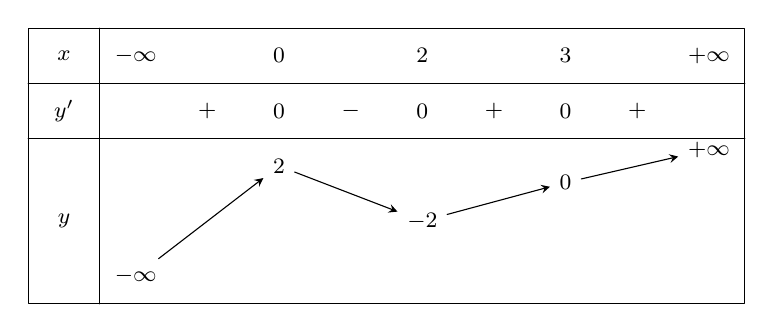
\begin{tikzpicture}[scale=0.7, font=\footnotesize, line join=round, line cap=round,>=stealth,yscale=1.0,xscale=1.3]
			\def\cot{9} % số nhãn chiều dài
			\def\hang{4} % số nhãn chiều cao
			\draw[shift={(-.5,.5)}] 
			(0,0) rectangle +(\cot+1,-\hang-1)
			(0,-1)--+(0:\cot+1) 
			(0,-2)--+(0:\cot+1) 
			(1,0)--+(-90:\hang+1);
			\path 
			(0,0) node{$x$}
			(1,0) node{$-\infty$}
			(3,0) node{$0$}
			(5,0) node{$2$}
			(7,0) node{$3$}
			(9,0) node{$+\infty$}
			(0,-1) node{$y'$}
			(2,-1) node{$+$}
			(3,-1) node{$0$}
			(4,-1) node{$-$}
			(5,-1) node{$0$}
			(6,-1) node{$+$}
			(7,-1) node{$0$}
			(8,-1) node{$+$}
			(0,-3) node{$y$} 
			(1,-4) node (dvcL) {$-\infty$}
			(3,-2) node (CTL) {$2$} 
			(7,-2.3) node (CTR) {$0$}  
			(5,-3) node (CD) {$-2$} 
			(9,-1.7) node (dvcR) {$+\infty$} ;
			\draw[->] (dvcL)--(CTL);
			\draw[->] (CTL)--(CD);
			\draw[->] (CD)--(CTR);
			\draw[->] (CTR)--(dvcR);
		\end{tikzpicture}
	\end{center}
	\choiceTF
	{\True Giá trị lớn nhất của hàm số $y=f(x)$ trên khoảng $(-\infty;2)$ là $2$}
	{$f\left(\cos^2 x\right)<f\left(\dfrac{3}{2}\right)$}
	{\True Hàm số $y=f(x)$ có hai cực trị}
	{Hàm số $g(x)=2x-3f(x)$ nghịch biến trên khoảng $(0;2)$}
	\loigiai{
		\begin{itemchoice}			
			\itemch
			Từ bảng biến thiên, ta có $\max\limits_{(-\infty;2)}f(x)=f(0)=2$.
			\itemch
			Ta có $0 \leq \cos^2 x \leq 1$.\\
			Trên $(0;2)$ hàm số nghịch biến nên $f\left(\cos^2x\right) \geq f(1)>f\left(\dfrac{3}{2}\right)$.
			\itemch
			Từ bảng biến thiên, hàm số có hai cực trị.
			\itemch
			Ta có $g(x)=2x-3f(x)$, $g'(x)=2-3f'(x)>0$, $\forall x \in(0;2)$ nên $g(x)$ đồng biến trên $(0;2)$.
		\end{itemchoice}
	}
\end{ex}
\begin{ex}%[2D1H5-3]%[KNTT - Lớp 12 - Dự án C - Đợt 4]%[Thanh Phong]%[GVPB Nguyễn Sĩ Đạt]
	Cho hàm số $y=f(x)=\dfrac{x^2-x+2}{x-2}$ có đồ thị $(C)$.
	\choiceTF
	{\True Đồ thị $(C)$ có tiệm cận đứng là đường thẳng $x=2$}
	{\True Đường thẳng $y=x+1$ là tiệm cận xiên của đồ thị hàm số}
	{Đồ thị $(C)$ đi qua điểm $M(0;1)$}
	{\True Có đúng $3$ giá trị $m$ nguyên thuộc đoạn $\left[0;10\right]$ để đường thẳng $y=m$ cắt đồ thị $(C)$ tại hai điểm phân biệt}
	\loigiai{
		\begin{itemchoice}			
			\itemch
			Tập xác định $\mathscr{D}=\mathbb{R} \setminus \{2\}$.\\
			$\lim\limits_{x\to 2^{+}}f(x)=+\infty$ nên đồ thị $(C)$ có tiệm cận đứng là đường thẳng $x=2$.
			\itemch
			$y=\dfrac{x^2-x+2}{x-2}=x+1+\dfrac{4}{x-2}$ nên $y=x+1$ là tiệm cận xiên của đồ thị hàm số.
			\itemch
			Với $x=0$ suy ra $y=-1$. Vậy điểm $(0;-1)\in (C)$.
			\itemch
			$y'=\dfrac{x^2-4 x}{(x-2)^2}$.\\
			$y'=0 \Leftrightarrow\hoac{&x=0\\&x=4.}$\\
			Ta có bảng biến thiên
			\begin{center}
				
\begin{tikzpicture}
					\tkzTabInit[espcl=3,lgt=1.5,nocadre]
					{$x$/0.7,$f'(x)$/0.7,$f(x)$/2.1}
					{$-\infty$,$0$,$2$,$4$,$+\infty$}
					\tkzTabLine{,+,0,-,d,-,0,+,}
					\tkzTabVar{-/$-\infty$,+/$-1$,-D+/$-\infty$/$+\infty$,-/$7$,+/$+\infty$}
				\end{tikzpicture}
			\end{center}
			Đường thẳng $y=m$ cắt $(C)$ tại hai điểm phân biệt khi và chỉ khi $m>7$ hoặc $m<-1$.\\
			Vì $m$ là số nguyên thuộc $[0;10]$ nên $m \in\{8,9,10\}$.
		\end{itemchoice}
	}
\end{ex}
\begin{ex}%[2D4V2-1]%[KNTT - Lớp 12 - Dự án C - Đợt 4]%[Thanh Phong]%[GVPB Nguyễn Sĩ Đạt]
	Gọi $F(x)$, $G(x)$ là nguyên hàm của $f(x)$. Hàm số $y=f(x)$ liên tục trên $\mathbb{R}$.
	\choiceTF
	{\True $\forall x \in \mathbb{R}$, $k\cdot F(x)$ là một nguyên hàm của $k\cdot f(x)$}
	{$\displaystyle\int\limits_a^bf(x)\mathrm{\,d}x=G(a)-G(b)$}
	{$F(x)-G(x)=0$, $\forall x \in \mathbb{R}$}
	{\True Cho $F(1)-5G(2)=3$ và $F(2)-5G(1)=15$. Giá trị $\displaystyle\int\limits_1^2f(x)\mathrm{\,d}x=2$}
	\loigiai{
		\begin{itemchoice}			
			\itemch
			Vì $(k\cdot F(x))'=k\cdot F'(x)=k\cdot f(x)$.
			\itemch
			Vì $\displaystyle\int\limits_a^bf(x)\mathrm{\,d}x=G(b)-G(a)$.
			\itemch
			Vì $F(x)-G(x)=C_1-C_2,\forall x \in \mathbb{R}$.
			\itemch
			Theo khái niệm tích phân  $\displaystyle\int\limits_1^2f(x)\mathrm{\,d}x=F(2)-F(1)=G(2)-G(1)$.\\
			Ta có $F(1)-5G(2)=3$ và $F(2)-5G(1)=15$. Suy ra
			\begin{eqnarray*}
				& & F(2)-F(1)+5[G(2)-G(1)]=12\\
				&\Leftrightarrow& \displaystyle\int\limits_1^2f(x)\mathrm{\,d}x+5\displaystyle\int\limits_1^2f(x)\mathrm{\,d}x=12\\
				&\Leftrightarrow& 6\displaystyle\int\limits_1^2f(x)\mathrm{\,d}x=12\\
				&\Leftrightarrow& \displaystyle\int\limits_1^2f(x)\mathrm{\,d}x=2.
			\end{eqnarray*} 
		\end{itemchoice}
	}
\end{ex}
\TNSA
\begin{ex}%[2D4H2-6]%[Đề thi thử môn Toán chuyenQuangTrung-BinhPhuoc-năm học 2025-2026]%[Lê Hùng Thắng - Nguyễn Sĩ Đạt]% 
	Trong một thí nghiệm sinh học, người ta theo dõi sự phát triển của một khối tế bào ung thư trong môi trường nuôi cấy. Ban đầu, khối tế bào có $1000$ tế bào. Sau $1$ ngày và sau $4$ ngày kể từ khi bắt đầu theo dõi, số lượng tế bào ung thư lần lượt là $1250$ tế bào và $2600$ tế bào. Gọi $N$ là số lượng tế bào ung thư tại thời điểm $t$ ngày $(0\le t\le 10 )$. Người ta ước tính tốc độ tăng trưởng của khối tế bào được mô tả bởi $N'(t)=at+b\sqrt{t}$, trong đó $a, b$ là các hằng số. Hỏi sau $8$ ngày, số lượng tế bào ung thư của khối tế bào là bao nhiêu? (kết quả làm tròn đến hàng đơn vị)
	
	\shortans{$4588$}
	\loigiai{
		Ta có $N(t )=\displaystyle\int\left(at+b\sqrt{t} \right)\mathrm{\,d}t=\dfrac{at^2}{2}+\dfrac{2}{3}bt\sqrt{t}+C$.\\
		Theo đề, ta có hệ $\heva{
			& N(0)=\dfrac{a\cdot 0^2}{2}+\dfrac{2}{3}b\cdot 0\sqrt{0}+C=1000 \\ 
			& N(1)=\dfrac{a\cdot 1^2}{2}+\dfrac{2}{3}b\cdot 1\sqrt{1}+C=1250 \\ 
			& N(4)=\dfrac{ac\dot 4^2}{2}+\dfrac{2}{3}b\cdot 4\sqrt{4}+C=2600 \\ 
		}\Leftrightarrow \heva{
			& a=-100 \\ 
			& b=450 \\ 
			& c=1000.}$\\
		Vậy sau $8$ ngày, số lượng tế bào ung thư của khối tế bào là \\
		$N(8)=\dfrac{-100\cdot.8^2}{2}+\dfrac{2}{3}\cdot 450\cdot 8\sqrt{8}+1000\approx 4588$.
} \end{ex} 

\begin{ex}%[1D6V3-5]%[Đề thi thử môn Toán chuyenQuangTrung-BinhPhuoc-năm học 2025-2026]%[Lê Hùng Thắng - Nguyễn Sĩ Đạt]%  
	Một nguồn âm đẳng hướng phát ra từ điểm $O$. Mức cường độ âm tại điểm $M$ cách điểm $O$ một khoảng $R$ ($R>0$) được tính bởi công thức $L_M=\log \dfrac{k}{R^2}$, với $k>0$ là hằng số. Biết điểm $O$ thuộc đoạn thẳng $AB$ và mức cường độ âm tại $A$ và $B$ lần lượt là $L_{A}=4{,}3$ (Ben) và $L_{B}=4{,}7$ (Ben). Mức cường độ âm tại trung điểm của $AB$ bằng bao nhiêu Ben? (kết quả làm tròn đến hàng phần chục)
	\shortans{$5,8$}
	\loigiai{
		Gọi $R_{A}$, $R_{B}$ lần lượt là khoảng cách từ $A$ và $B$ đến $O$ ($x\in \mathbb{N}$).\\
		Ta có $\heva{
			& {{L}_{A}}=4,3 \\ 
			& {{L}_{B}}=4,7}
		\Leftrightarrow \heva{
			& \log \dfrac{k}{R_{A}^2}=4,3 \\ 
			& \log \dfrac{k}{R_{B}^2}=4,7}
		\Leftrightarrow \heva{
			& \dfrac{k}{R_{A}^2}=10^{4,3} \\ 
			& \dfrac{k}{R_{B}^2}=10^{4,7}.}$\\
		Khi đó khoảng cách từ $O$ tới trung điểm $M$ của $AB$ bằng $R_M=\dfrac{R_{A}-R_{B}}{2}$ (vì $R_A > R_B$).\\
		Mức cường độ âm tại trung điểm của $AB$ bằng \\
		$L_{M}=\log\dfrac{k}{{R_M}^2}=\log \dfrac{k}{\left(\dfrac{R_{A}-R_{B}}{2}\right)^2}\\
		=\log \dfrac{4}{\dfrac{R_{A}^2}{k}-2\cdot \dfrac{R_{A}\cdot R_{B}}{k}+\dfrac{R_{B}^2}{k}} \\ 
		=\log \dfrac{4}{\dfrac{1}{{{10}^{4{,}3}}}-2\sqrt{\dfrac{1}{10^{4{,}3}\cdot\dfrac{1}{10^{4{,}7}}}}+\dfrac{1}{10^{4{,}7}}}\approx 5{,}8.\\ 
		$
	}
\end{ex} 

\begin{ex}%[0D8V2-6]%[Đề thi thử môn Toán chuyenQuangTrung-BinhPhuoc-năm học 2025-2026]%[Lê Hùng Thắng - Nguyễn Sĩ Đạt]%  
	\immini[thm]{Một khu đô thị có mạng lưới giao thông được mô hình hóa là một lưới ô vuông mà mỗi ô vuông có cạnh độ dài $1$ đơn vị như hình vẽ, mỗi tuyến phố trong khu đô thị được coi là $1$ cạnh của ô vuông đơn vị, trong khu đô thị có $2$ cái hồ, hồ số $1$ nằm trong $4$ ô vuông, hồ số $2$ nằm trong $6$ ô vuông như hình vẽ. Một anh Shipper đang ở địa điểm $A$ và cần đi giao hàng ở địa điểm $B$. Hỏi anh Shipper có bao nhiêu cách đi biết rằng anh Shipper chỉ có thể đi sang phải hoặc đi xuống về phía $B$.
	}
	{\begin{tikzpicture}[scale=0.71,>=stealth, font=\footnotesize, line join=round, line cap=round]
			\draw(0,0) grid (6,5);
			\fill[pattern=north east lines,opacity=0.5](0,1) rectangle(3,3);
			\fill[pattern=north east lines,opacity=0.5](4,2) rectangle(6,4);
			\fill[white] (1.5,2) circle (0.7) node [black] {HỒ 2};
			\fill[white] (5,3) circle (0.7) node [black] {HỒ 1};
			\node at (0,5)[above left] {$A$};
			\node at (6,0)[below right] {$B$};
		\end{tikzpicture}
	}
	\shortans{$204$}
	\loigiai{
		Chọn điểm xuất phát $A$ làm gốc tọa độ $(0;0)$.\\
		Trục $Ox$ hướng sang phải. Trục $Oy$ hướng xuống dưới. Khi đó $B(6;5)$. Ta có\\
		+ Số đường đi bất kỳ (kể cả đi qua điểm nằm trong hồ) từ điểm $A$ đến điểm $B$ là $\mathrm{C}_{11}^5=462$ cách.\\
		+ Số đường đi qua điểm $M(1;3)$ $(A\rightarrow M\rightarrow B)$ là: $\mathrm{C}_4^1\cdot \mathrm{C}_7^5=84$ cách.\\
		+ Số đường đi qua điểm $N(2;3)$ $(A\rightarrow N\rightarrow B)$ là: $\mathrm{C}_5^2\cdot \mathrm{C}_6^4=150$ cách.\\
		+ Số đường đi qua điểm $T(5;2)$ $(A\rightarrow P\rightarrow B)$ là: $\mathrm{C}_7^5\cdot \mathrm{C}_4^1=84$ cách.\\
		+ Số đường đi qua cả $M(1;3)$ và $N(2;3)$ $(A\rightarrow M\rightarrow N\rightarrow B)$ là: $\mathrm{C}_4^1.1\cdot \mathrm{C}_7^5=60$ cách.\\
		Vậy số đường đi hợp lệ là: $462-(84+150+84-60)=204$ cách.
	} 
\end{ex} 

\begin{ex}%[1H8V5-3]%[Đề thi thử môn Toán chuyenQuangTrung-BinhPhuoc-năm học 2025-2026]%[Lê Hùng Thắng - Nguyễn Sĩ Đạt]%  
	Cho hình chóp $S.ABCD$ có đáy là hình chữ nhật, cạnh $AB=2AD=2$. Tam giác $SAB$ đều và nằm trong mặt phẳng vuông góc với mặt phẳng đáy $(ABCD)$. Tính khoảng cách từ điểm $A$ đến mặt phẳng $(SBD)$ (kết quả làm tròn đến hàng phần trăm).
	\shortans{$0,87$}
	\loigiai{
		\begin{center}
			\begin{tikzpicture}[>=stealth,line join=round,line cap=round,font=\footnotesize,scale=0.8]
				\path (0,0) coordinate (A)
				(-2,-1.6) coordinate (B)
				(4,0) coordinate (D)
				($(B)+(D)-(A)$) coordinate (C)
				($(A)!0.5!(B)$) coordinate (H)
				($(H)+(0,3)$) coordinate (S)
				(intersection of A--C and B--D) coordinate (O);
				\draw (S)--(B)--(C)--(D)--(S)--(C);
				\draw[dashed] (B)--(A)--(D)--(B) (O)--(H)--(S)--(A)--(C);
				\foreach \d/\g in {A/180,B/-135,C/-45,D/0,S/90,O/-95,H/-90} \fill (\d)node[shift={(\g:0.3)}]{$\d$} circle(1pt);
			\end{tikzpicture}
		\end{center}
		Gọi $H,O$ lần lượt là trung điểm của $AB,BD$.\\
		Ta có: $SH\perp AB$ (do tam giác $SAB$ đều), $OH\perp HB$, $HB=1$, $HO=\dfrac{1}{2}$, $HS=\sqrt{3}$.\\
		Mà mặt phẳng $(SAB)\perp(ABCD)$, $(SAB)\cap(ABCD)=AB$ nên $SH\perp (ABCD)$.\\
		Suy ra $HS\perp HO$, $HS\perp HB$.\\
		Ta có $\dfrac{\mathrm{d}(A,(SBD) )}{\mathrm{d}(H,(SBD))}=\dfrac{BA}{BH}=2\Rightarrow \mathrm{d}(A,(SBD) )=2\mathrm{d}(H,(SBD))=2\mathrm{d}(H,(SBO))$.\\
		Mặt khác $HS, HO, HB$ đôi một vuông góc nên ta có:\\
		$\dfrac{1}{{{d}^2}( H,(SBO) )}=\dfrac{1}{H{{B}^2}}+\dfrac{1}{H{{O}^2}}+\dfrac{1}{H{{S}^2}}=\dfrac{16}{3}$.\\
		Vậy $\mathrm{d}(A,(SBD))=2\mathrm{d}(H,(SBO))=2\cdot\dfrac{\sqrt{3}}{4}=\dfrac{\sqrt{3}}{2}\approx 0,87$.
	}
\end{ex} 
\begin{ex}%[2D1V5-8]%[Đề thi thử môn Toán chuyenQuangTrung-BinhPhuoc-năm học 2025-2026]%[Lê Hùng Thắng - Nguyễn Sĩ Đạt]%  
	Doanh nghiệp A chế biến và bán ra thị trường sản phẩm điều thành phẩm. Giả sử khi sản xuất và bán hết $x$ tấn sản phẩm (với $0<x\le 100$) thì tổng số tiền doanh nghiệp thu được được biểu thị bởi hàm số $f(x)=200x-x^2$ (đơn vị triệu đồng) và tổng chi phí mà doanh nghiệp chi ra biểu thị bởi hàm số $g(x)=x^2+140x+5$ (đơn vị triệu đồng). Ngoài ra khi bán $1$ tấn sản phẩm doanh nghiệp còn phải chịu mức thuế phụ thu là $m$ (đơn vị triệu đồng), (với $0<m<50$). Tìm giá trị của $m$ sao cho nhà nước nhận được số tiền thuế phụ thu lớn nhất và doanh nghiệp cũng thu được lợi nhuận lớn nhất theo mức thuế phụ thu đó.
	\shortans{$30$}
	\loigiai{
		Tổng số tiền thuế thu được khi bán $x$ tấn sản phẩm là $h( m )=mx$.\\
		Tổng lợi nhuận mà doanh nghiệp thu được khi bán $x$ đơn vị sản phẩm là \\
		$t(x)=f(x)-g(x)-h(m)=-2x^2+(60-m)x-5\Rightarrow t'(x)=-4x+60-m$. \\ 
		$t'(x)=0\Leftrightarrow x=\dfrac{60-m}{4}$.\\
		Nhận thấy để $t(x)$ lớn nhất khi $x=\dfrac{60-m}{4}$.\\
		Khi đó tổng số tiền thuế thu được khi bán $x$ tấn sản phẩm là\\
		$h( m )=mx=\dfrac{60m-{{m}^2}}{4}\Rightarrow h'(m)=\dfrac{60-2m}{4}$.\\
		$h'( m )=0\Leftrightarrow m=30$.\\
		Bảng biến thiên
		\begin{center}
			\begin{center}
				
\begin{tikzpicture}
					\tkzTabInit[nocadre=false,lgt=1.2,espcl=2.5,deltacl=0.6]
					{$m$ /0.6,$h'(m)$ /0.6,$h(m)$ /2}
					{$0$,$30$,$50$}
					\tkzTabLine{,+,$0$,-,}
					\tkzTabVar{-/$ $, +/$h(30)$,-/$ $}
				\end{tikzpicture}
			\end{center}
		\end{center}
		Từ bảng biến thiên của hàm số $h(m)\Rightarrow h(m)$ lớn nhất khi $m=30$.
	} 
\end{ex} 

\begin{ex}%[2H5V2-8]%[Đề thi thử môn Toán chuyenQuangTrung-BinhPhuoc-năm học 2025-2026]%[Lê Hùng Thắng - Nguyễn Sĩ Đạt]%  
	\immini[thm]{Trong một căn phòng có một bức tranh hình tròn trên tường bán kính bằng $2$ m, tâm của bức tranh cách mặt đất $3$ m và cách bức tường còn lại $4$ m. Người ta thiết lập hệ trục tọa độ $Oxyz$ (như hình vẽ). Một thợ trang trí nhận thiết kế đường hiệu ứng, xuất phát từ điểm $A$ ở mép tường cách bức tường treo bức tranh $6$ m, đến điểm $B$ trên bức tường treo bức tranh theo phương $\overrightarrow{u}=( 2;-3;3)$ và nối đến điểm $C$ trên đường tròn của bức tranh. Hỏi tổng độ dài ngắn nhất của đường hiệu ứng bằng bao nhiêu mét? (Kết quả làm tròn đến chữ số thập phân hàng phần chục)
	}
	{
		\begin{tikzpicture}[x={(-0.85cm,-0.45cm)}, y={(0.7cm,-0.15cm)}, z={(0cm,1cm)},	line cap=round, line join=round, >=stealth, font=\footnotesize, scale=0.5]
			%!<\usetikzlibrary{calc,arrows.meta,3d}>
			% Định nghĩa tham số dựa trên đề bài
			\def\R{2}      % Bán kính tranh
			\def\zI{3}     % Tâm I cách mặt đất (z)
			\def\xI{4}     % Tâm I cách tường bên (x)
			
			% Tường treo tranh nằm trong mặt phẳng y = 0
			\coordinate (O) at (0,0,0);
			\coordinate (I) at (\xI, 0, \zI); % Tâm bức tranh
			\coordinate (A) at (0, 6, 0);     % A trên trục Oy, cách tường y=0 là 6m
			
			% Tính tọa độ điểm B:
			% B nằm trên tường y=0 => y_B = 0.
			% Phương trình tham số đường thẳng qua A(0,6,0) véc tơ u(2,-3,3):
			% x = 0 + 2t; y = 6 - 3t; z = 0 + 3t.
			% Cho y=0 => 6 - 3t = 0 => t = 2.
			% Suy ra B = (4, 0, 6).
			\coordinate (B) at (4, 0, 6);
			
			% Tính tọa độ điểm C trên đường tròn (I, R) sao cho BC ngắn nhất:
			% C là giao điểm của đoạn thẳng BI với đường tròn.
			% BI = sqrt((4-4)^2 + (0-0)^2 + (6-3)^2) = 3.
			% Vì BI > R (3 > 2) nên C nằm giữa B và I.
			% Độ dài BC = BI - R = 3 - 2 = 1.
			\coordinate (C) at (4, 0, 5);
			
			% --- VẼ HÌNH KHÔNG GIAN ---
			
			% Vẽ các mặt tường (Painter's algorithm: vẽ từ sau ra trước)
			% Sàn nhà
			\fill[gray!15] (0,0,0) -- (0,7,0) -- (5,7,0) -- (5,0,0) -- cycle;
			% Tường x=0 (Tường bên)
			\fill[pink!22] (0,0,0) -- (0,7,0) -- (0,7,7) -- (0,0,7) -- cycle;
			% Tường y=0 (Tường treo tranh)
			\fill[blue!12] (0,0,0) -- (6,0,0) -- (6,0,7) -- (0,0,7) -- cycle;
			
			% Vẽ khung lưới sàn (tùy chọn để tạo chiều sâu)
			\draw[blue!50, thin] (0,0,0) grid[step=1] (0,7,7);
			\draw[blue!80, thin] (0,0,0) grid[step=1] (6,0,7);
			
			% Vẽ bức tranh tròn (nằm trên tường y=0)
			\begin{scope}[canvas is xz plane at y=0]
				\draw[thick, fill=blue!10, opacity=0.6] (\xI, \zI) circle (\R);
				\node at (\xI, \zI) [above left] {$I$};
			\end{scope}	
			% Vẽ hệ trục tọa độ Oxyz
			\draw[->, blue, thick] (O) -- (7,0,0) node[below left] {$x$};
			\draw[->, blue, thick] (O) -- (0,8,0) node[below right] {$y$};
			\draw[->, blue, thick] (O) -- (0,0,8) node[left] {$z$};
			\node[blue, below] at (O) {$O$};
			
			% Vẽ đường hiệu ứng A -> B -> C
			\draw[thick] (A) -- (B) -- (C);
			
			% Đánh dấu các điểm nút
			\fill[red] (A) circle (2.5pt) node[above right, black] {$A$};
			\fill[red] (B) circle (2.5pt) node[above, black] {$B$};
			\fill[red] (C) circle (2.5pt) node[above left, black, xshift=-1mm] {$C$};
			\fill[black] (I) circle (1.5pt);
			
		\end{tikzpicture}
	}
	\shortans{$10,4$}
	\loigiai{
		Ta có $I(4;0;3)$. Bức tranh là đường tròn $(C)$ tâm $I$, bán kính $R = 2$ nằm trong mặt phẳng $(Oxz)$.\\
		Điểm $A$ nằm ở mép tường (trên trục $Oy$) và cách bức tường treo tranh (mặt phẳng $Oxz$) $6$ m $\Rightarrow A(0; 6; 0)$.\\
		Đường thẳng $\Delta$ đi qua $A(0; 6; 0)$ và có vectơ chỉ phương $\vec{u} = (2; -3; 3)$ có phương trình là\\
		$\heva{
			& x=2t \\ 
			& y=6-3t \\ 
			& z=3t}$ suy ra $B( 2t;6-3t;3t)$. \\
		Mà điểm $B$ nằm trên bức tường treo tranh (mặt phẳng $Oxz$) nên\\ $y_{B}=0\Rightarrow 6-3t=0\Rightarrow t=2\Rightarrow B(4;0;6)$.\\
		$\Rightarrow AB=2\sqrt{22}$.\\
		Tổng độ dài đường hiệu ứng là $S = AB + BC$.\\
		Vì $AB$ không đổi nên $S$ nhỏ nhất khi khoảng cách $BC$ là nhỏ nhất.\\
		Ta thấy $B(4;0;6)$ và đường tròn $(C)$ đều cùng nằm trong mặt phẳng $(Oxz)$ ($y=0$). \\
		Bài toán trở thành bài toán hình học phẳng trong mặt phẳng tọa độ $(Oxz)$.\\
		$BI=\sqrt{(4-4)^2+(6-3)^2}=3 > 2=R$ nên điểm $B$ nằm ngoài đường tròn $(C)$.\\
		Suy ra, điểm $C$ nằm trên đường tròn $(C)$ sao cho $BC$ ngắn nhất khi $C$ là giao điểm của đoạn thẳng $BI$ với đường tròn. \\
		Khi đó $BC_{\min}=BI-R=1$.\\
		Tổng độ dài ngắn nhất của đường hiệu ứng là: $S_{\min}=AB+B\mathrm{C}_{\min}=2\sqrt{22}+1\approx 10{,}4$ m.
	}
\end{ex}

\Closesolutionfile{ans}
